\par A dualidade onda-partícula de um elemento na escoala atômica é uma propriedade básica descrita pela mecânica quântica\cite{qm_fis3}. Quando as partículas são tratadas como ondas, a função de onda ($\Psi$) é utilizada para formalizar seu deslocamento e amplitude\cite{qm_fis4}. A densidade de probabilidade, $\left| \Psi \right|^2$, é utilizada quando se deseja encontrar a probabilidade de uma partícula estar em um determinado local.

    \par Para conseguir descrever um sistema quântico matematicamente, Erwin Schrödinger desenvolveu a principal equação em torno da mecânica quântica, conhecida como equação de Schrödinger, que está escrita a seguir:

    \begin{equation}\label{eq_schrodinger_main}
      \mathcal{H} \cdot \Psi(\mathbf{r}) = \left[ -\frac{\hbar^2}{2m}\nabla^2 + U(\textbf{r}) \right] \cdot \Psi(\mathbf{r}) = \Psi(\mathbf{r})
    \end{equation}

    \par Na equação \eqref{eq_schrodinger_main}, $\mathcal{H}$ é o operador hamiltoniano - que será melhor explorado mais a frente- e o termo $ -\frac{\hbar^2}{2m}\nabla^2 $ é o operador momento, no qual $\nabla^2$ é o Laplaciano que representa a segunda derivada. Além disso, U(\textbf{r}) é o potencial da partícula numa dada posição \textbf{r}.

    \par O termo E é a energia da partícula no estado que ela se encontra, sendo um autovalor na equação de Schrödinger que está associado ao autovetor da função de onda.

    \par Para analisar a energia do elétrons, a partícula será confinada em um poço de potencial infinito, unidimensional em x = [0,L]. Será considerado que a partícula move-se livremente e que não há brechas na barreira de potencial, evitando assim o tunelamento quântico. Reescrevendo a equação (2.0) para o caso unidimensional e explicitando as condições de contorno:

    \begin{equation}\label{eq_schrodinger_frustrado}
      -\frac{\hbar^2}{2m} \nabla^2 \Psi(x) + U(x) \cdot \Psi(x) = E \cdot \Psi(x),
      \ onde\ V(0)=V(L)=\infty\ e\ V(x)=0,\ 0<x<a
    \end{equation}

    Onde, podemos escrever ainda

    \begin{equation}\label{eq_schrodinger_eq1}
      \Psi(\mathbf{x}) = \left(\frac{1}{L}\right)^\frac{1}{2} sen\left(\frac{n \cdot \pi \cdot x}{L}\right),\ com\ n = 1, 2, ...
    \end{equation}

    \par Sendo n o número quântico relacionado com o nível de energia em que a partícula se encontra. Pode-se verificar uma equação de onda bem definida (autovetor) para cada valor de nível de energia do sistema (autovalor), exemplificado na figura \ref{fig1}\cite{frustrado2}.

    \begin{figure}[h!]
      \caption{Formas da função de onda para valores de n entre 1 e 6}
      \centering
      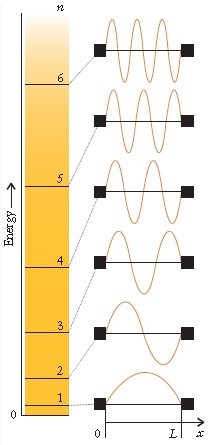
\includegraphics[width=0.25\textwidth]{images/figura1.png}
      \label{fig1}
    \end{figure}

    \par Pela definição clássica da funçaõ de onda $\Psi(\mathbf{x})$, temos:

    \begin{equation}\label{eq_schrodinger_eq2}
        \Psi (\mathbf{x}) = A \cdot sen(k \cdot \mathbf{x}) + B \cdot cos(k \cdot \mathbf{x})
    \end{equation}

    %TODO - QUAIS CONDIÇÕES SÃO ESSAS?
    \par Pela equação de Schrödinger, \eqref{eq_schrodinger_eq2} e das condições de contorno para o problema em questão, é possível concluir:

    \begin{equation}\label{eq_schrodinger_eq3}
      E = \frac{\hbar^2}{8 \pi^2 m} \cdot \frac{n^2\pi^2}{L^2} = \frac{\hbar^2 n^2}{8 m L^2},\ com\ n = 1, 2, ...
    \end{equation}

    \par Como $n \in \mathcal{Z} - \{0\}$, a equação \eqref{eq_schrodinger_eq3} mostra que somente alguns valores para energia são aceitos no confinamento dentro de uma caixa de tamanho L. A partir disso, conclui-se que os níveis de energia de uma partícula confinada são discretos e que a energia pode ser quantizada\cite{frustrado2}.

    \par Para definir o operador hamiltoniano utilizado para descrever partículas num cristal, começaremos do cristal perfeito, que descreve de maneira geral as relações entre as partículas nesse sistema. A partir dele, serão feitas aproximações para que se chegue no hamiltoniano do elétron livre\cite{qm_fis2}.

    \subsubsection{Hamiltoniano de um Cristal Perfeito}

      \par Para definir o operador hamiltoniano utilizado para descrever partículas num cristal, começaremos do cristal perfeito, que descreve de maneira geral as relações entre as partículas nesse sistema. A partir dele, serão feitas aproximações para que se chegue no hamiltoniano do elétron livre\cite{qm_fis2}. 
    
      \par O hamiltoniano do cristal perfeito\cite{frustrado3} é dado por:
      %TODO - REVISAR
      \begin{equation}\label{eq_schrodinger_eq4}
        \mathcal{H} = 
          \sum_{i} \frac{p_{i}^2}{2m_{i}} 
          + \sum_{j} \frac{p_{j}^2}{2m_{j}} 
          + \frac{1}{2} \sum_{j', j} \frac{Z_{j} Z_{j'} e^2}{4\pi\epsilon_{0}\left|R_{j} - R_{j'}\right|}-  \sum_{j, i} \frac{Z_{j} e^2}{4\pi\epsilon_{0}\left|r_{i} - R_{j}\right|} 
          + \frac{1}{2} \sum_{i, i'} \frac{e^2}{4\pi\epsilon_{0}\left|r_{i} - r_{i'}\right|}
      \end{equation}

      \par Na expressão \eqref{eq_schrodinger_eq4}, $\epsilon_{0}$ representa a permissividade no vácuo, $r_{i}$ representa a posição do i-ésimo elétron, $R_{j}$ representa a posição do j-ésimo núcleo, $Z_{j}$ representa o número atômico do núcleo, $p_{i}$ e $p_{j}$ representam o operador momento dos elétrons e o operador momento do núcleo, respectivamente. Além disso, os índices $i'$ e $j'$ são índices não identicos a $i$ e $j$.

      \par Para solucionar o hamiltoniano, leva-se em conta que os elétrons nas camadas totalmente preenchidas estão muito próximos ao núcleo, considerando-os como um pacote. Essa junção de elétrons mais internos com o núcleo atômico forma o que se chama por íon-núcleo.
    
      \par A partir disso, serão aplicadas duas aproximações para facilitar a solução do hamiltoniano. A primeira será a aproximação de Born-Oppenheimer.\cite{qm_fis9}


      \par Essa aproximação divide os átomos em duas grandes regiões. A primeira região trata o núcleo como uma partícula estática no espaço. Já a segunda região lida somente com as partículas na superfície do sistema.

      \par Aplicando a aproximação de Born-Oppenheimer ao hamiltoniano, pode-se separar os cálculos entre os íons-núcleo e os elétrons na camada de valência. Assim, simplifica-se o hamiltoniano como uma soma de hamiltonianos da relação entre os elétrons de valências, entre os íons-núcleo e entre ambas regiões, da seguinte maneira:

      \begin{equation}\label{eq_schrodinger_eq5}
        \mathcal{H} = 
          \mathcal{H}_{ions} (\mathbf{R}_{j}) 
          + \mathcal{H}_{e}(\mathbf{r}_{i}, \mathbf{R}_{j_{0}})
          + \mathcal{H}_{e-ion}(\mathbf{r}_i, \delta\mathbf{R}_j)
      \end{equation}

      \par Nessa expressão, $\mathcal{H}_{ions}(\mathbf{R}_{j})$ é o hamiltoniano referente às interações entre os íons-núcleo que se movimentam devido aos seus potenciais iônicos; $\mathcal{H}_{e}(\mathbf{r}_{i},\mathbf{R}_{j_{0}})$ é o hamiltoniano referente às interações elétron-elétron, considerando os íons-núcleo estáticos e congelados na posição de equilíbrio $\mathbf{R}_{j_{0}}$; $\mathcal{H}_{e-ion}(\mathbf{r}_{i},\delta\mathbf{R}_{j})$ é o hamiltoniano que descreve a interação elétron-íon, caracterizando a variação na energia eletrônica causada pelo deslocamento $\delta\mathbf{R}_{j}$ dos íons-núcleo em relação ao seu ponto de equilíbrio $\mathbf{R}_{j_{0}}$.
      
      \par Escrevendo o hamiltoniano do cristal perfeito, retirando os termos referentes unicamente ao núcleo e mantendo as interações elétron-elétron, obtém-se:

      \begin{equation}\label{eq_schrodinger_eq6}
        \mathcal{H}_{e} = 
          \sum_{i} \frac{p_{i}^2}{2m_{i}} 
          -  \sum_{j, i} \frac{Z_{j} e^2}{4\pi\epsilon_{0}\left|r_{i} - R_{j_{0}}\right|} 
          + \frac{1}{2} \sum_{i, i'} \frac{e^2}{4\pi\epsilon_{0}\left|r_{i} - r_{i'}\right|}
      \end{equation}

      \par Para simplificar a equação \eqref{eq_schrodinger_eq6}, será utilizada a aproximação \textit{mean-field}\cite{qm_fis10}. Essa aproximação consiste na escolha de um local arbitrário para o elétron no sistema e na consideração de que os outros graus de liberdade se encontram estáticos se utilizarmos seu valor médio. Aplicando o hamiltoniano somente em um elétron, tem-se que:

      \begin{equation}\label{eq_schrodinger_eq7}
        \mathcal{H}_{1e} = \frac{p^2}{2m}
      \end{equation}

      Considerando que o operador momento,na mecânica quântica, é definido por\cite{qm_fis11}:

      \begin{equation}\label{eq_schrodinger_eq8}
        p = -i\hbar\frac{d}{dx} \Longrightarrow
        p^2 = -\hbar^2 \frac{d^2}{dx^2} \Longrightarrow
        p^2 = -\hbar^2 \nabla^2
      \end{equation}

      Aplicando \eqref{eq_schrodinger_eq8} em \eqref{eq_schrodinger_eq7}, tem-se:

      \begin{equation}\label{eq_schrodinger_eq9}
        \mathcal{H}_{1e} = - \frac{\hbar^2}{2m}\nabla^2
      \end{equation}

      Define-se assim, o operador hamiltonia para o caso considerado. Aplicando a equação de Schrödinger ao caso do elétron livre, no qual o potencial U(\textbf{r}) é igual a zero, tem-se que:

      \begin{equation}\label{eq_schrodinger_eq10}
        \mathcal{H} \cdot \Psi(\mathbf{r}) =
          -\frac{\hbar^2}{2m} \nabla^2 \Psi(\mathbf{r}) =
          E \cdot \Psi(\mathbf{r})
      \end{equation}

      Com autovalores de energia dados por:

      \begin{equation}\label{eq_schrodinger_autovalores}
        E = \frac{\hbar^2 k^2}{2m}
      \end{equation}

      Em uma rede cristalina, o elétron sofre influência de um potencial. Esse potencial pode ser tratado como um potencial periódico\cite{qm_fis5} em alguns casos e será explicado a seguir.